\section{Data augmentation} \label{app:data_aug}

\subsection{Decorrelating departure and arrival delays}
Inspecting the correlation matrix (Fig.~\ref{img:full_corr}), we notice an extremely high correlation between \texttt{Departure delay} and \texttt{Arrival delay}. This value makes the two variables almost duplicates of one another. In order to remove this redundancy while retaining as much information as possible, we decided to replace Arrival delay with a quantity that captures the difference between the two.

We considered two options:
\begin{itemize}
    \item using the plain difference between the two variables;
    \item fitting a simple linear regression model with \texttt{Arrival delay} as the target and \texttt{Departure delay} as the covariate, and taking the residual of each observation as the new covariate.
\end{itemize}
The second model is more general and, in fact, encompasses the first one; however, the first is more interpretable and carries an immediate meaning, such as ``mid-flight delay'' or ``time gained during the flight''. The deciding point was whether the second option differed enough from the first to justify its higher complexity.

The regression model that reproduces the plain difference is the one with slope equal to 1 and intercept equal to 0. Fitting the regression model on the full dataset yields an intercept of 0.76 and a slope of 0.97; we therefore decided to opt for the simple difference between the arrival and departure delays.

\subsection{Reducing covariates skewness}
From the boxplots in Fig.\ref{fig:boxplot_skew} we can see how covariates \texttt{Flight Distance}, \texttt{Departure Delay} and \texttt{Mid-flight delay} are extremelly right-skewed. Since covariate skewnes might slow down MCMC convergence and are prone to present outliers and leverage points, we decided to transform them and check whether the transformation is beneficial.
\begin{figure}[h]
    \centering
    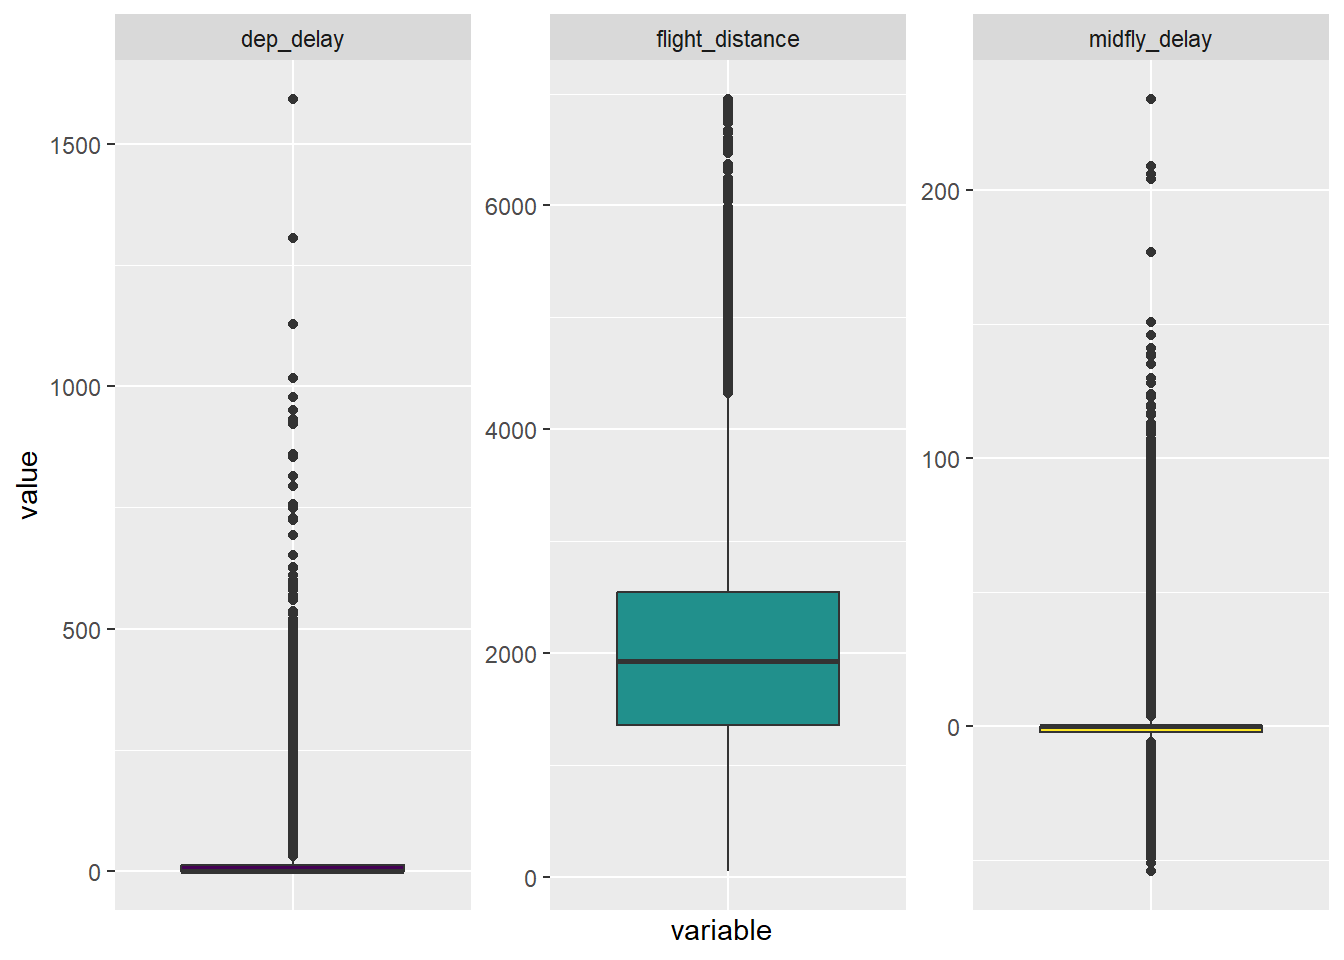
\includegraphics[width=0.5\linewidth]{img//data_expl/boxplot_skew.png}
    \caption{Boxplots of skewed covariates.}
    \label{fig:boxplot_skew}
\end{figure}

Since both \texttt{Flight distance} and \texttt{Departure delay} are non-negative we transform them using $ln(1+x)$; instead for \texttt{Mid-flight delay} we use the \textit{signed-log transformation} $\text{sign}(x)    \cdot ln(1+|x|)$ due the presence of negative values.
\begin{table}[ht]
\centering
\begin{tabular}{lr}
\hline
\textbf{variable} & \textbf{skewness} \\
\hline
Flight Distance & 0.466 \\
log1p(Flight Distance) & -1.599 \\
Departure Delay & 6.853 \\
log1p(Departure Delay) & 0.919 \\
Midflight Delay & 2.941 \\
signed-log(Midflight delay) & 0.234 \\
\hline
\end{tabular}
\caption{Skewness of raw and transformed variables}
\label{tab:skewness}
\end{table}

As we can see in Tab.~\ref{tab:skewness} \texttt{Flight distance} is only midly skewed and the transformation actually turn to be worse than the original varibale, therefore we kept it unchanged. Instead for what concerns \texttt{Departure delay} and \texttt{Mid-flight delay} we see higher level of skewness and the transformation improves this aspect; therefore we decided to kee the log-transformed variables.

